\section{Evaluation}
\label{Evaluation}
As mentioned in Section~\ref{benchmarking}, the following data has been collected using my custom-made \emph{benchlat} utility. For this final benchmark, each algorithm was executed 500 times for 3, 4, and 5 anchors. The anchors were placed at random positions close to distinct borders of the playing area. For each set of anchors, the original implementation of each algorithm was executed as well in order to obtain a reference runtime. The achieved speed-up of each anchor/algorithm combination was calculated using the formula $s = \frac{t_{r}}{t_{o}}$, where $t_{o}$ denotes the optimized runtime and $t_{r}$ is the reference runtime. The average speed-up was then derived using the usual formula for the arithmetic mean that is displayed in Formula~\ref{eq:arithmetic_mean}.
\begin{equation}
\label{eq:arithmetic_mean}
\texttt{avg}(S) = \frac{1}{n} \cdot \sum_{i = 1}^n s_{i}
\end{equation}

\begin{table}
\begin{center}
\begin{tabular}{lccc} 
\toprule
& \multicolumn{3}{c}{Average speed-up} \\ 
\cmidrule(r){2-4}
Algorithm & 3 anchors & 4 anchors & 5 anchors \\
\midrule
AML & 2.70 & 2.91 & 3.01 \\
GEO3 & 2.20 & 2.22 & 2.18 \\ 
VBLE-OPT & 1.64 & 1.77& 1.75 \\
\bottomrule
\end{tabular}
\caption{Average speed-ups}
\label{average_table}
\end{center}
\end{table}


\begin{figure}[ht]
\begin{center}
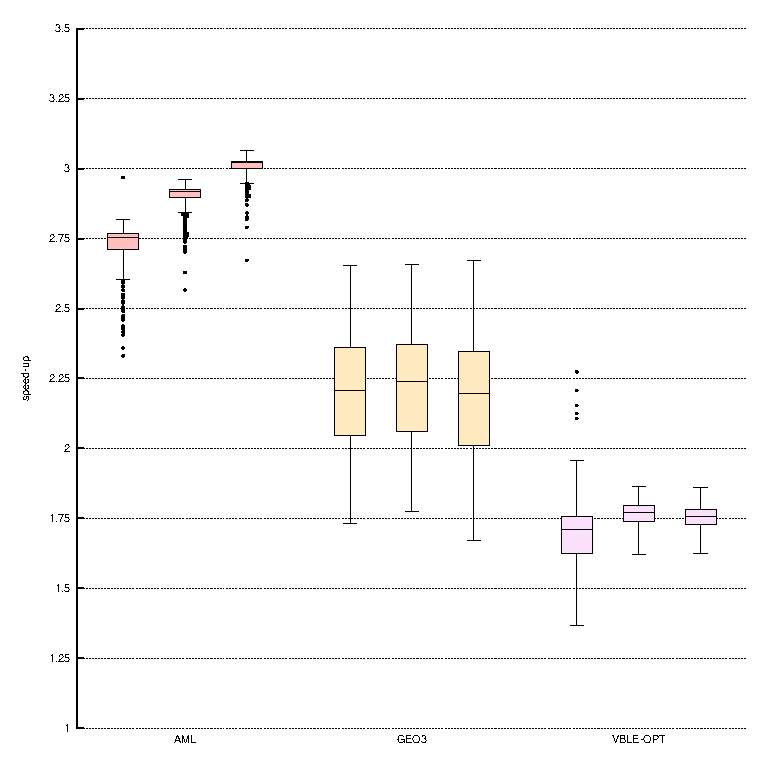
\includegraphics[width=14cm]{img/boxplot}
\end{center}
\caption{Distribution of speed-ups}
\label{fig:boxplot}
\end{figure}